
There exist two design approaches to the problem of measuring the deuteron EDM inside a storage ring:
\begin{enumerate*}[(i)]
	\item the Frozen Spin (FS) lattice, and
	\item the Quasi-frozen spin (QFS) lattice.
\end{enumerate*}

In the following sections we will consider variants of both type lattices.

\subsection{The Frozen Spin lattice} \label{chpt2:lattice:FS_BNL}
In an FS-type lattice, the horizontal projection of a beam particle's spin vector is 
\emph{continuously} aligned with its momentum vector. In order to realize the continuity condition, 
combined E+B-field cylindrical spin-rotators are inserted into the accelerator arc sections. 
An example of a FS-type lattice~\cite{Senichev:Lattices} is shown in Figure~\ref{fig:BNL_lattice}. 
This ring is 145.85~m in length and is designed for the deuteron beam injection energy 270~MeV. 
An RF cavity is used in order to suppress linear spin decoherence effects by time-averaging 
the beam particles' kinetic energies.
The RF voltge used is $V = 100$~kV, RF frequency $f_{RF} = 5\cdot f_{rev}$,
where the cyclotron frequency $f_{rev} = 1.00$~MHz. The remaining non-linear decoherence effects are
suppressed by means of three~\footnote{Some authors use two families~\cite{Eremey:Thesis} in this lattice.}
sextupole families.

\begin{figure}[h!]
	\centering
	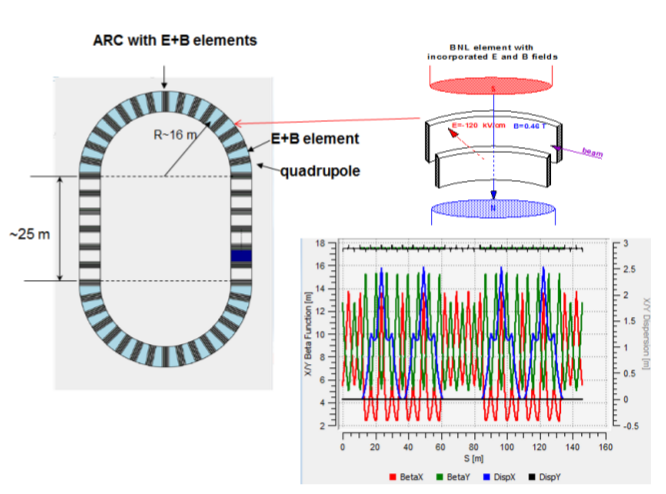
\includegraphics[width=\linewidth]{images/chapter2/BNL_lattice}
	\caption{A FS lattice variant. Cylindrical E+B spin-rotators are used in the arc sections to fulfill
          the continuous FS condition. (Image is taken from~\cite{Senichev:Lattices}.)\label{fig:BNL_lattice}}
\end{figure}

The main purpose of the FS lattice design is to maximize the EDM signature signal. 
However, it is important to note that, strictly speaking, the FS condition is fulfilled only 
for the reference particle. This is because, as follows from
equation~\eqref{eq:TBMT_MDM}, for any given E- and B-fields there exists a unique value of 
the Lorentz factor $\gamma$ at which $\W_y^{MDM} = 0$. Hence, even in a FS lattice, 
most particles' spin vectors are frozen only approximately.

\subsection{Quasi-Frozen Spin lattice} \label{chpt2:concept:QFS}
In the QFS design concept, one gives up the continuity property of the FS state, 
requiring only that the spin phase advance (in the rest frame) in the electrostatic ($\Phi_s^E$) 
and magnetic ($\Phi_s^B$) elements was zero on average (at each turn):~\cite{Senichev:Lattices}
\begin{equation*}
	\sum_i \Phi_{s,i}^E = -\sum_j \Phi_{s,j}^B.
\end{equation*}

Following the definition of spin tune (see section~\ref{sec:TBMT_introduction}), a particle's spin vector
placed into an electromagnetic field turns by angle $\Phi_s = \nu_s \cdot \Phi$, where $\Phi$ is
the momentum angle of turn, $\nu_s$ spin tune.

A particle's angular momentum, when placed into a magnetic field $\vec B$ is
\[
\w_B = \frac qm \frac B \gamma,
\]
into an electrostatic $\vec E$:
\[
\w_E = \frac qE \frac{\vec E\times \vec\beta}{c\beta^2\gamma},
\]
from which follow the expressions for spin tune in the electrostatic and magnetic fields:
\begin{equation}
	\begin{cases}
		\nu_s^B &= \gamma G, \\
		\nu_s^E &= \beta^2\gamma\bkt{\frac{1}{\gamma^2-1} - G}.
	\end{cases}
\end{equation}

The QFS lattice design has the advantage of simplicity over the FS one: there's no need to use a combined-field
cylindrical spin rotators; in both QFS lattice variants we consider below are used either
\begin{enumerate*}[(i)]
\item straight Wien filters,  or
\item cylindrical electrostatic and magnetic elements separately.
\end{enumerate*}
On the other hand, due to the appearance of a vertical spin precession axis component $\bar n_y$,
the maximum EDM signal amplitude is less compared with the pure FS case. The attenuation
factor~\cite{Senichev:QFS_IPAC15}
\[
J_0(\Phi_s) \approx 1 - \frac{\Phi_s^2}{4},
\]
where $\Phi_s$ is the maximum horizontal plane spin phase advance. 

Assume the phase advance does not exceed $\pi\cdot \gamma G/2n$; in this context $n$ is 
the lattice periodicity. Since the deuteron anomalous magnetic moment $G = -0.142$, $J_0\ge 0.98$ for the QFS lattices considered below.

\subsubsection{QFS lattice design ``6.3''}\label{chpt2:lattice:QFS:6_3}

A QFS design lattice~\cite{Senichev:Lattices} in which E- and B-fields are separated in space
is presented in Figure~\ref{fig:QFS_6_3_lattice}. Negative radius electrostatic cylindrical deflectors 
are used to compensate the spin phase advance related to the MDM precession in the
 arc sections.~\cite{Senichev:QFS_IPAC15}
The ring is 166.67~m length long and is designed for 270~MeV injection energy. For the suppression
of linear spin decoherence effects, an RF cavity is used, with voltage $V = 100$~kV, and operating
frequency $f_{RF} = 5\cdot f_{rev}$, where $f_{rev} = 0.87$~MHz. Non-linear decoherence effects are suppressed
means of six sextupole families.

\begin{figure}[h!]
	\centering
	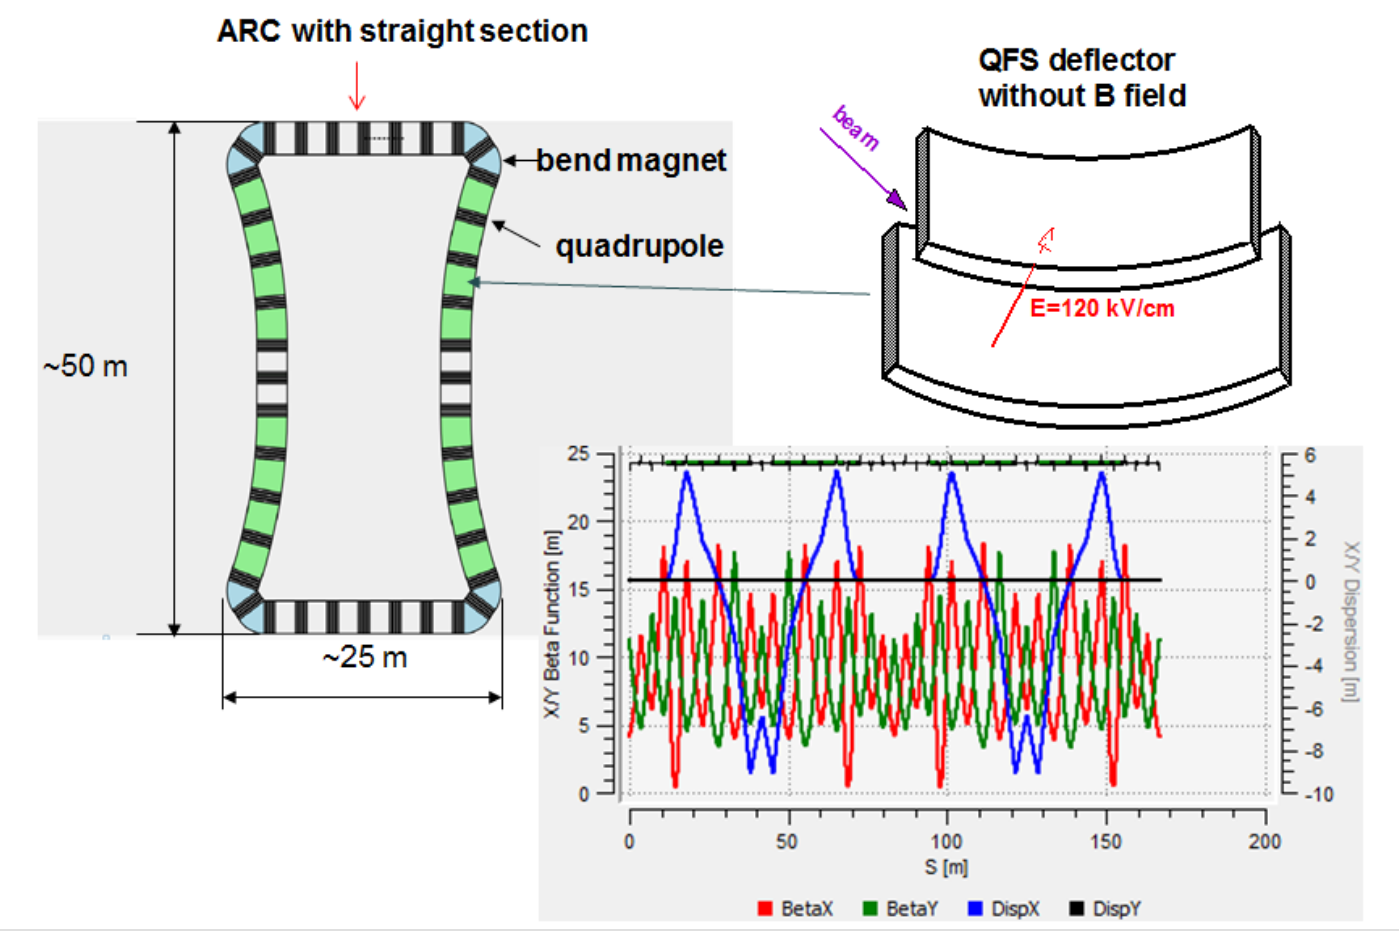
\includegraphics[width=\linewidth]{images/chapter2/6_3_lattice}
	\caption{QFS lattice design variant with spatially separated E- and B-fields.
          (Image taken from~\cite{Senichev:Lattices})\label{fig:QFS_6_3_lattice}}
\end{figure}

\subsubsection{QFS lattice design ``E+B''}\label{chpt2:lattice:QFS:EB}

The lattice design in Figure~\ref{fig:QFS_E+B_lattice} utilizes plain, straight, static Wien filters.
This allows one to:
\begin{enumerate*}[\itshape a\upshape)]
	\item exclude non-linear electrostatic field components present in curved electrostatic fields, and 
	\item simplify the lattice from the engineering point of view.
\end{enumerate*}

The lattice is 149.21~m in length, the injection energy is 270~MeV. 
The linear spin decoherence effects suppressing RF cavity has a longitudinal voltage $V = 100$~kV, 
and frequency $f_{RF} = 5\cdot f_{rev}$, with $f_{rev} = 0.98$~MHz. 
Four sextupole families are used in the suppression of non-linear decoherence effects.
\begin{figure}[h!]
	\centering
	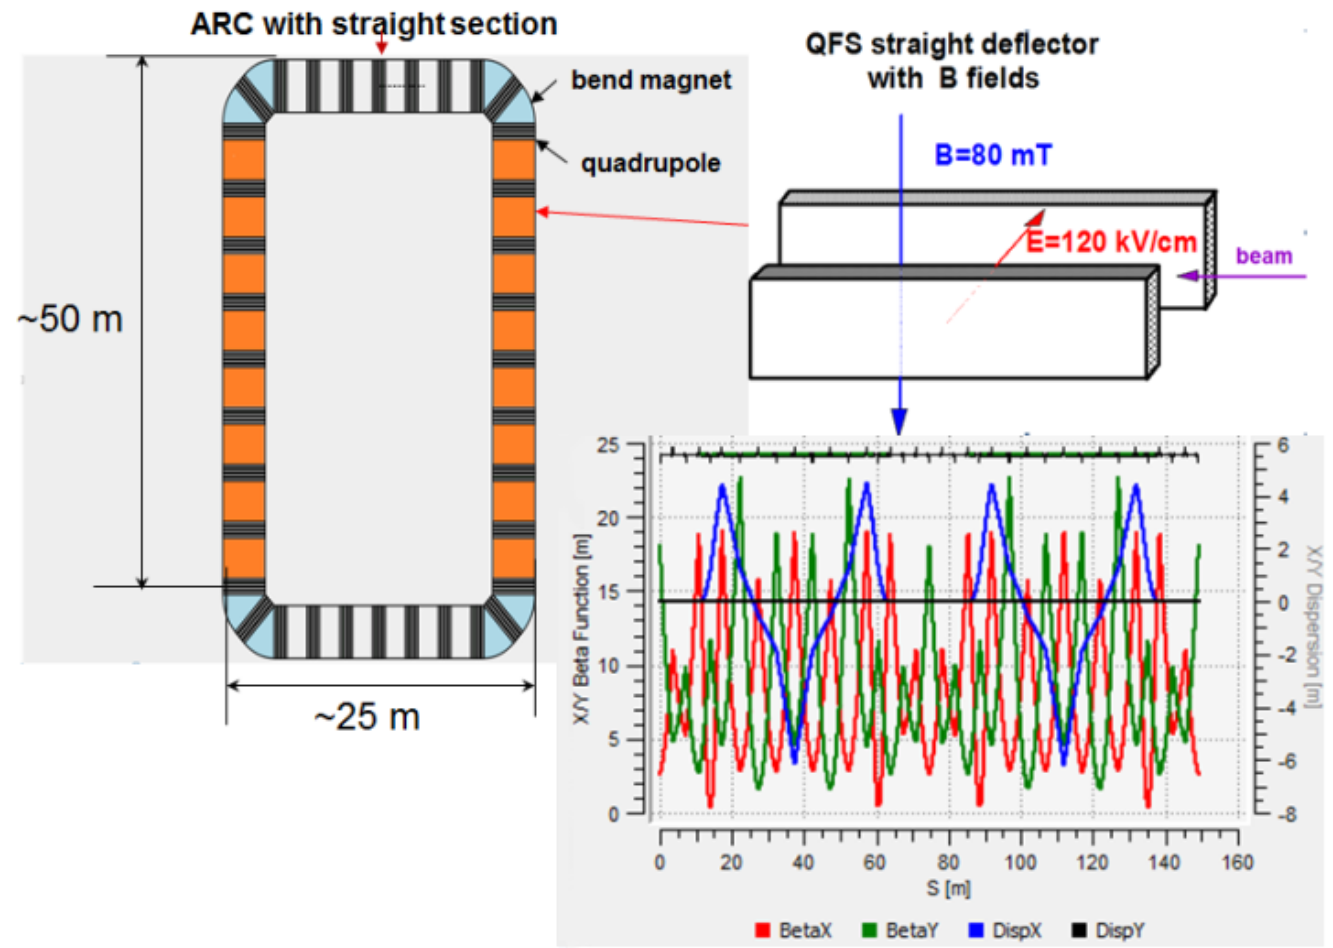
\includegraphics[width=\linewidth]{images/chapter2/E+B_lattice}
	\caption{Straight Wien filters QFS lattice variant.
          (Image taken from~\cite{Senichev:Lattices})\label{fig:QFS_E+B_lattice}}
\end{figure}

